\documentclass[main.tex]{subfiles}

\usepackage{tikz}
\usetikzlibrary{positioning}

\begin{document}

\thispagestyle{empty}

\begin{center}
\Large
Дополнительное задание №2\\
Нотная запись (вариант 22)
\end{center}

\vspace{1cm}

\begin{center}
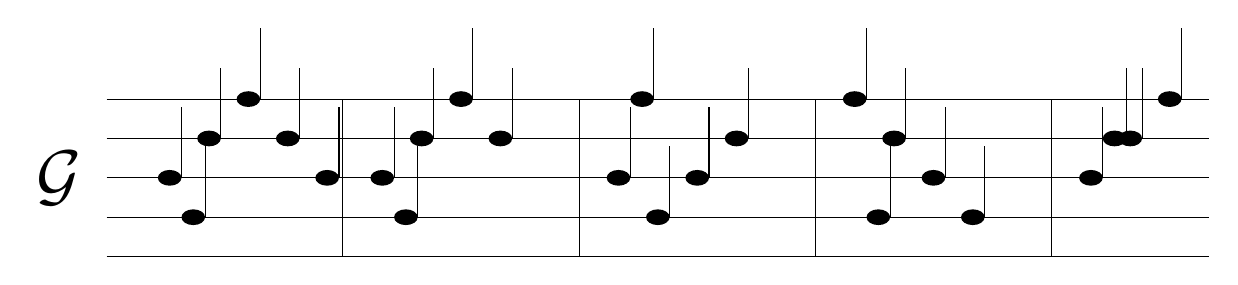
\begin{tikzpicture}[scale=1]

% Нотный стан (5 линий)
\foreach \y in {0,0.5,1,1.5,2} {
    \draw (0,\y) -- (14,\y);
}

% Скрипичный ключ (упрощённо)
\node at (-0.6,1) {\Huge $\mathcal{G}$};

% Тактовые черты
\foreach \x in {3,6,9,12} {
    \draw (\x,0) -- (\x,2);
}

% Ноты (более 25 штук)
\foreach \x/\y in {
0.8/1,1.3/1.5,1.8/2,2.3/1.5,
3.5/1,4/1.5,4.5/2,5/1.5,
6.5/1,7/0.5,7.5/1,8/1.5,
9.5/2,10/1.5,10.5/1,11/0.5,
12.5/1,13/1.5,13.5/2,
1.1/0.5,3.8/0.5,6.8/2,
9.8/0.5,12.8/1.5,2.8/1
}
{
    \fill (\x,\y) ellipse (0.15 and 0.1);
    \draw (\x+0.15,\y) -- (\x+0.15,\y+0.9);
}

\end{tikzpicture}
\end{center}

\vfill

\begin{center}
\textit{Ноты выполнены средствами LaTeX с использованием пакета TikZ}
\end{center}

\end{document}
